% Created 2022-10-25 Tue 08:04
\documentclass[9pt, b5paper]{article}
\usepackage{xeCJK}
\usepackage{minted}
\usepackage[T1]{fontenc}
\usepackage[scaled]{beraserif}
\usepackage[scaled]{berasans}
\usepackage[scaled]{beramono}
\usepackage{graphicx}
\usepackage{xcolor}
\usepackage{multirow}
\usepackage{multicol}
\usepackage{float}
\usepackage{textcomp}
\usepackage{algorithm}
\usepackage{algorithmic}
\usepackage{latexsym}
\usepackage{natbib}
\usepackage{geometry}
\geometry{left=1.2cm,right=1.2cm,top=1.5cm,bottom=1.2cm}
\newminted{common-lisp}{fontsize=\footnotesize} 
\usepackage[xetex,colorlinks=true,CJKbookmarks=true,linkcolor=blue,urlcolor=blue,menucolor=blue]{hyperref}
\author{deepwaterooo}
\date{\today}
\title{游戏基本场景设计}
\hypersetup{
  pdfkeywords={},
  pdfsubject={},
  pdfcreator={Emacs 27.1 (Org mode 8.2.7c)}}
\begin{document}

\maketitle
\tableofcontents

\begin{itemize}
\item debugging game flow, 现游戏的主场景如下(看起来很丑,但它运行!!!):
\end{itemize}

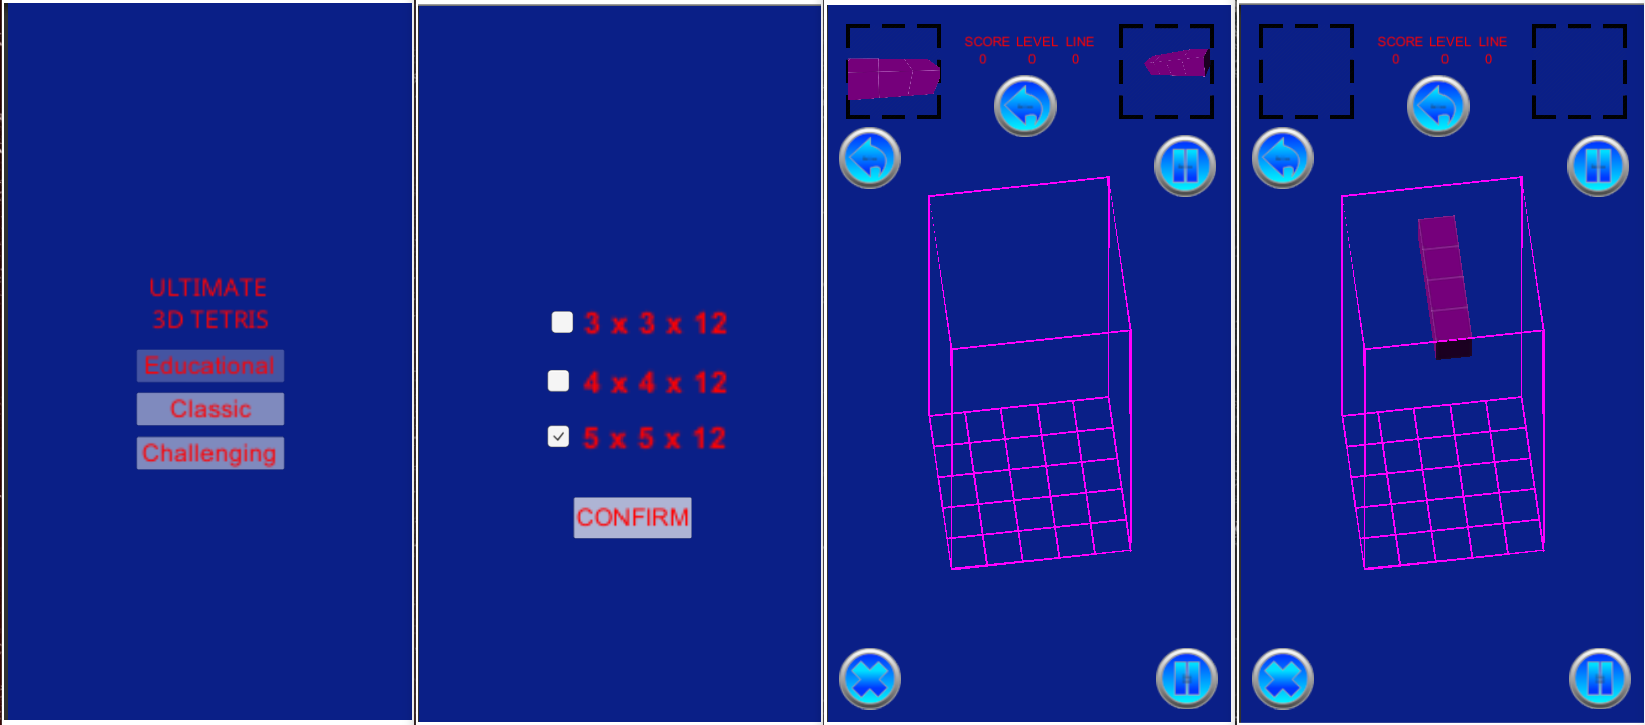
\includegraphics[width=.9\linewidth]{./pic/readme_20221022_223927.png}
\begin{itemize}
\item 预设都做好了,现在要将预设打资源包,并从资源包读出来供视图实例化等
\item finding the easist way to refactor yet still be able to hotfix after app installed already.
\item 现在游戏显示都没有问题了,开始debug 游戏逻辑以及功能模块等(现在只是运行了可模拟测试版的,需要在热更新程序域里将这些逻辑重构到运行出这种效果来,明天写,明天下午写?还是什么时候来写这点儿呢?)
\begin{itemize}
\item trying to link all necessary game logics and make game to run again in ILRuntime HotFix 程序域里.
\end{itemize}
\item \textbf{TODO:}
\item 继续现在改好的逻辑,把游戏逻辑连起来.基本现在能够想到的比较难一点儿的全都连通了,狠开心,爱表哥,爱生活!!!
\item 昨天平移和旋转画布上的两组按钮的点击事件没有问题;可是今天UI面板上有些按钮点不通,这个点击事件的传递系统,也还需要花点时间.热更新程序域里的绝大部分按钮都是点得通可以回调的,平移组四个按钮,旋转组应该也没有问题,主游戏界面暂停按钮也可以好好工作,只是有些按钮还连不能,感觉是其它问题. (同类按钮,同一面板上的按钮,能够有一个可以运行,那么这个大的框架逻辑是通的,就不用担心了,剩余只将是细节上的小修改)
\item 现在最主要的逻辑有以上两个问题.但都能够解决.(两个基本都解决了!!!强大的debugging strategy!!! 爱表哥, 爱生活!!!)
\begin{itemize}
\item <Tetromino> <GhostTetromino> 继承自MonoBehaviour的脚本在运行时添加适配过程中出意外: instance总是空,也可以说是我的AddComponent<T>方法没有适配?这个类型的适配有点儿没有做好(这个应该是目前最重要的问题,但不是不能解决的问题)把官方DEMO中的例子好好运行好研究透彻再来试图解决自己目前遇到的问题(两个项目可以参考)
\item 我不知道现存的方案里其它人的项目是如何实现的.回到问题的本质,那就变成为最简单的办法, 便是自己实现一个计时系统,或是模拟一个每隔(比如说1秒钟,方块砖就下降一格就可以了,that's it!)这次重构想要达到的目标便是基本绝大部分的逻辑都可以热更新重构.那么只要我能够模拟每隔一秒更新一次就解决问题了,这个项目对于我来说80\%逻辑理顺,剩下的就是热更新的服务器了
\item 自己实现计时器的方法大致思路:那就分section,每个小节玩5分钟,挑战模式可以加到10分钟;每个方块砖每隔两秒下降一格;需要考虑应用的离线时间,就是游戏过程中去玩别人的应用了,再回来时间连续计算一个小节5分钟
\item 今天下午理过思路包括:
\begin{itemize}
\item 刚才没有把问题想明白:因为经过了适配,本身的UnityEngine.AddComponent<T>() UnityEngine.GetComponent<T>() 在热更新工程中的正常运行是没有问题的
\begin{itemize}
\item 出问题的特殊之处是在: Tetromini.cs GhostTetromino.cs是在热更新工程中定义的,当游戏运行,unity工程无法得知热更新工程中Tetromino.cs GhostTetromino.cs为何物
\item 上面说得不对,因为加component本身是在热更新工程中,它是知道自己工程中所定义的部件的
\end{itemize}
\item 所以得想办法把这两个类移到Unity工程中来(这个反而可能会比较繁琐,也可能逻辑不通)
\item 按照官方建议,我们是可以重置这两个方法的,让它有办法认得热更新工程中所定义的脚本(顺着这条途径把问题理顺,那么就发现别人的控件逻辑是在Unity主工程的,也就是有主工程中的MonoBehaviour系来驱动各生命周期事件,但是我的热更新控制逻辑是在热更新工程中,并没有一个默认的游戏引擎来驱动事件的自行发生)
\item 所以,没有设置好的原因,另一个是在热更新工程中,我没有哪个地方来调用UNITY工程的系统的自动运行;
\begin{itemize}
\item 前面的各种适配是适配给unity,让它认识热更新工程中的诸多类型函数等
\item 可是按照自己游戏逻辑,感觉更像是热更新工程中需要适配unity MonoBehaviour的生命周期事件 ?
\item 那么再回到上面,刚想过的
\end{itemize}
\item 所以得想办法把这两个类移到Unity工程中来(这个反而可能会比较繁琐,也可能逻辑不通)
\begin{itemize}
\item 那么这么试一下,倒还是有可能的,unity MonoBehaviour系能够自动驱动生命周期事件,引导必要时候游戏的进行 ??? 测试一下
\end{itemize}
\end{itemize}
\end{itemize}

\item 示例工程中这些劫持是,代码适配用于提供给Unity工程来加载或是获取(AddComponent<>(), GetComponent<>())热更新工程中unity所不认识的定义的类等,与自己游戏逻辑不同,不用        

\begin{itemize}
\item AudioManager,EventManager可能需要适配,就需要自己把原理都弄明白了
\item 先前的PoolManager的解决是采用ViewManager里静态管理的方法,可以如期运行,有待优化
\item 那么上面两个如果一时半会儿找不到更好的办法,就可以参照上面的方法解决
\end{itemize}
\end{itemize}

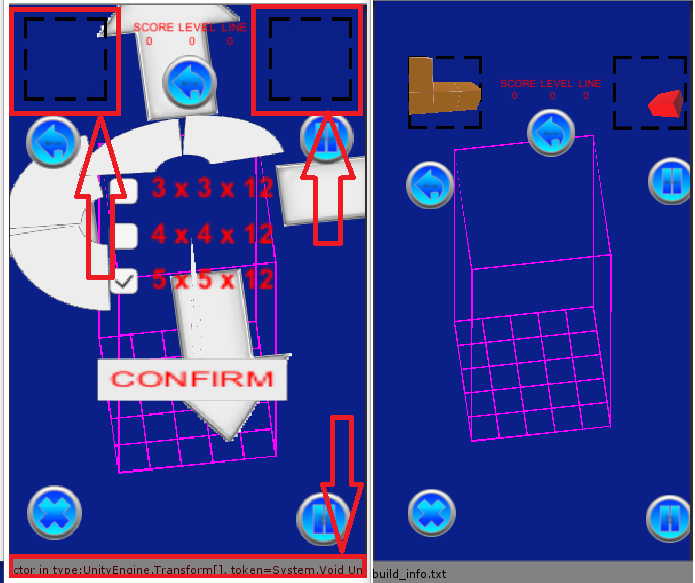
\includegraphics[width=.9\linewidth]{./pic/readme_20221020_195727.png}
\begin{itemize}
\item \textbf{已经解决了的先前的}
\begin{itemize}
\item moveCanvas rotateCanvas上点击事件,事件系统的传递.如果上面的问题一时半会儿解决不了,可以先试图解决这个并测试一下,给上面最难的BUG一点儿网络搜索和解决问题的时间 (狠好解决)这里只是用了最基础的方法来实现,以前自己都曾实现过事件系统,现在只是测试和解决主要关键点,知道都可行可实现,会再进一步的使用适当的设计模式来优化源码
\item 两个预览方块砖的生成并画到视图上去: 现在解决这个问题
\begin{itemize}
\item 原理很简: 将两个预览放在不会出现在主相机的两个固定的位置上;再用两个不同的相机分别照在两个预览上,并分别投射到一块渲染媒介,显示在屏幕的固定投影位置上就可以了
\item 大致原理如此,但运行时存在:场景里各不同视图会被某些不确定的因素旋转某些角度,以及放大缩小位数的问题.
\item 运行时可能涉及这块投影渲染媒介的实例化(不知道目前不能很好地渲染是否是因为我打包时没有打包它?还是说因为他们出现在两个不同视图的原因呢?)
\item 就是因为如上的目前我还不太理解的不确定性,给这个游戏的unity视图显示造成一定的困难,但也不是都解决不了的,需要花时间来慢慢解决这些小问题
\end{itemize}
\end{itemize}
\item at least temporatorily passed inital running 
\begin{itemize}
\item 现两个主要的小问题:多维数组在ILRuntime热更新程序域里的适配,
\item 多维数组,稍微改动了一下就可以了,但里面还是有点儿小机关的
\begin{itemize}
\item AOT不能使用二维数组(多维数组)例如bool[,]e
\item 使用时报System.Boolean[,]::Get没有生成AOT代码
\item 改用bool[][]是OK的
\item ILRuntime Version
\item 1.6.7
\item 答案是: 需要正确生成clr绑定
\end{itemize}
\end{itemize}
\item 热更新里重新实现在的游戏主场景如下:
\end{itemize}

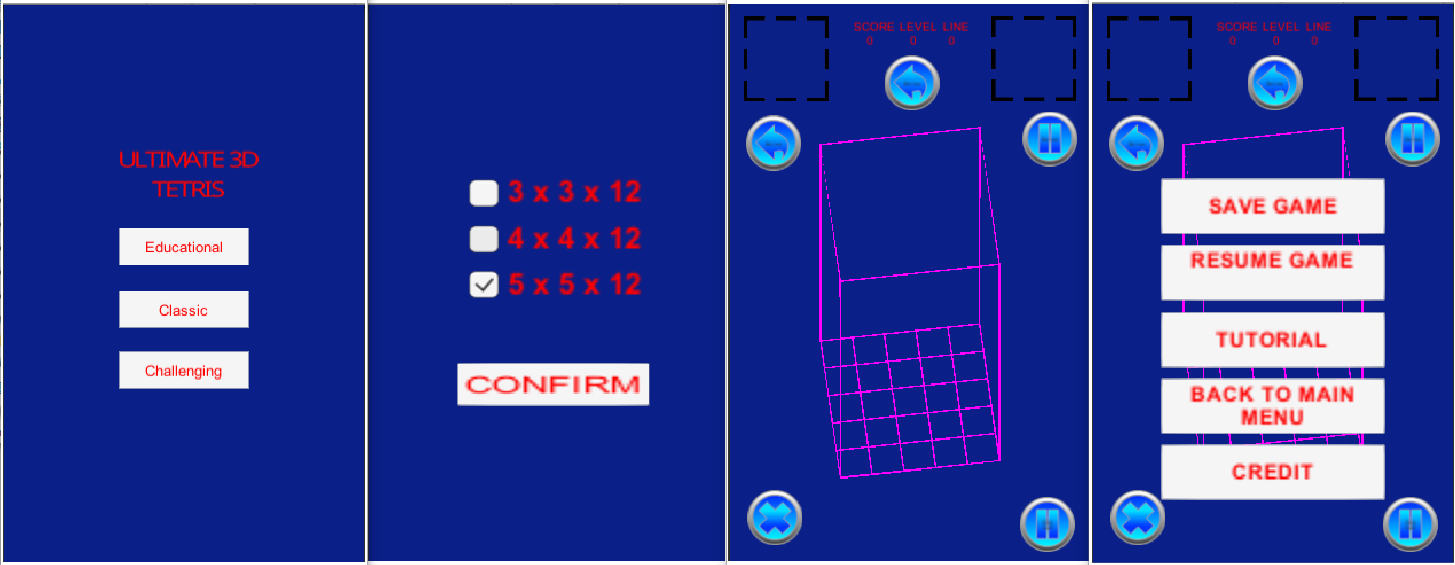
\includegraphics[width=.9\linewidth]{./pic/readme_20221011_201317.png} 
\begin{itemize}
\item 主游戏菜单与游戏过程中选择菜单: 最右为Educational has 3 choices:
\end{itemize}

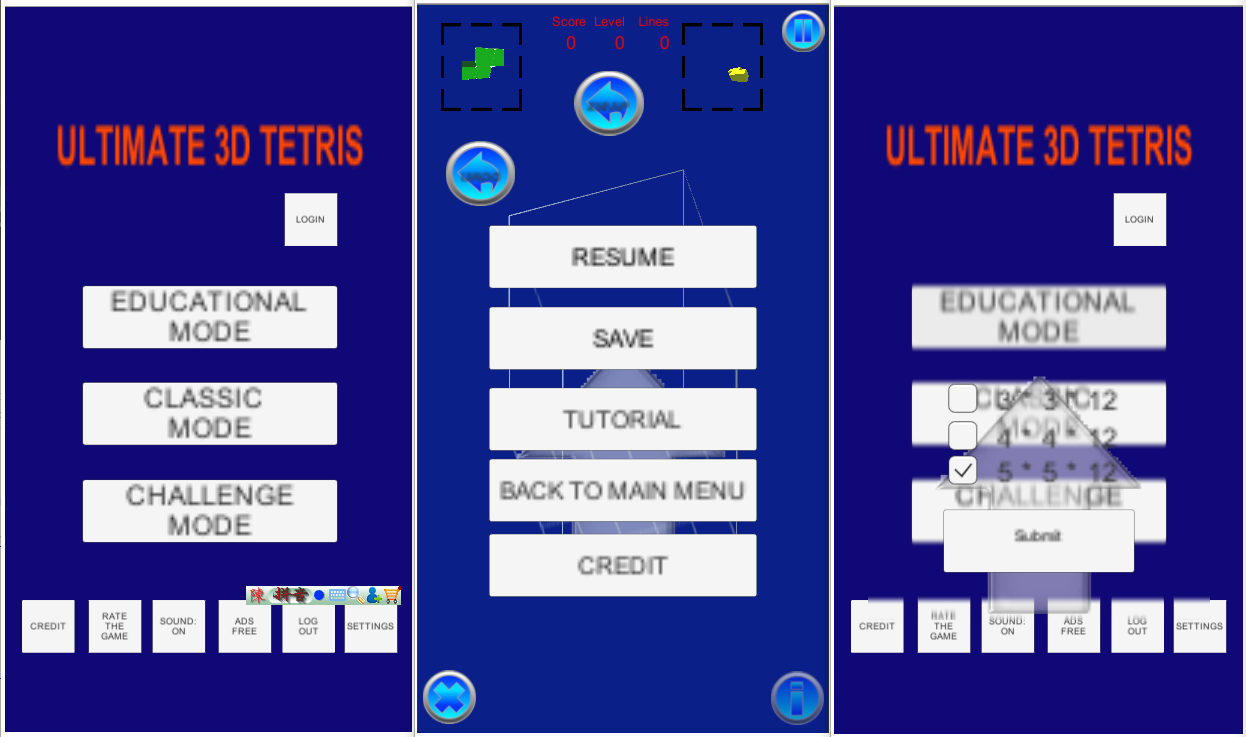
\includegraphics[width=.9\linewidth]{./pic/readme_20221007_192732.png}
\begin{itemize}
\item 启蒙模式原本是想给小盆友玩儿的,有无限撤销方块功能,和粒子消除行与列。但是这具模式有可能最终被我砍掉,相关功能改加到其它模块 
\item 启蒙模式下的由易到难三种选择:Educational mode的三种不同界面
\end{itemize}

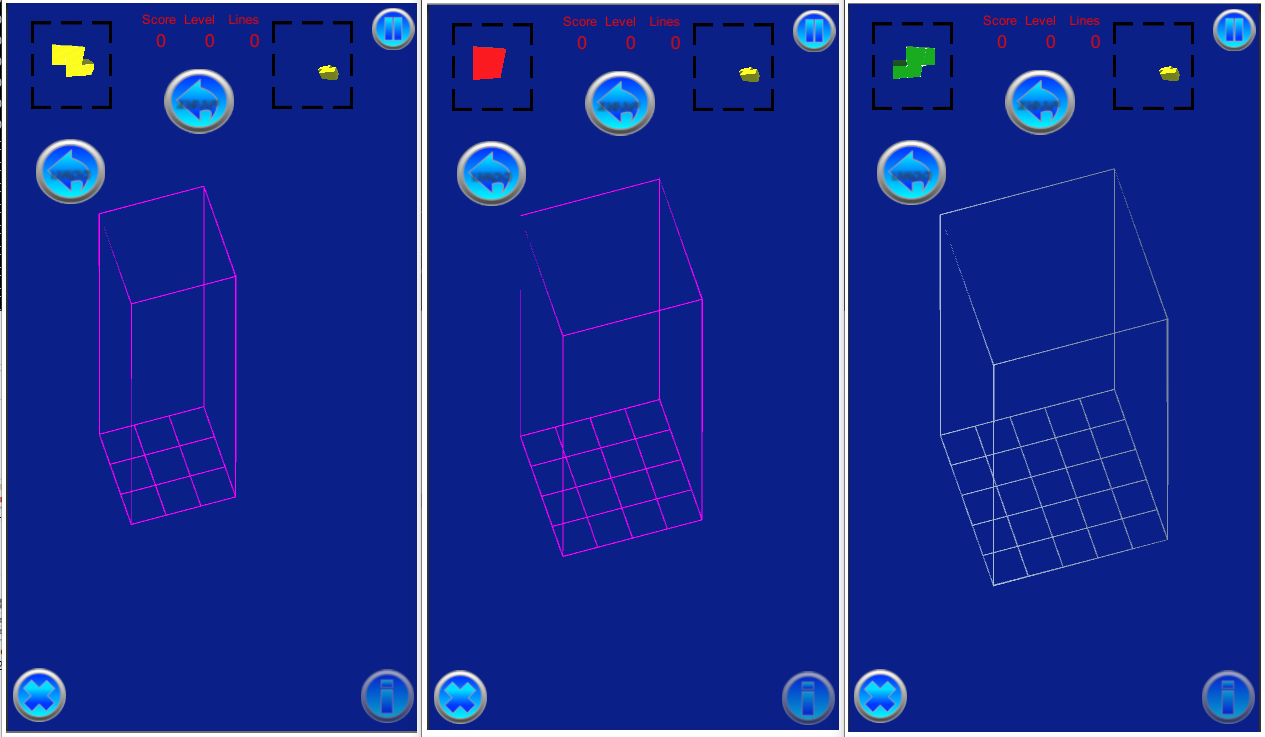
\includegraphics[width=.9\linewidth]{./pic/readme_20222007_193727.png}

\begin{itemize}
\item 传统游戏界面视图:(挑战模式下的界面丢了,到时候再补吧,或者可能只做7级,剩余热更新)
\item 两组共10个对各小方块砖方块砖平移与旋转的操纵:  \textbf{平移与旋转按钮都太丑,的摆放与位置需要优化}
\item load new game or saved games: 保存游戏数据的地址需要再改变一下,改变到应用的内部,而不是要存到什么其它的盘
\end{itemize}

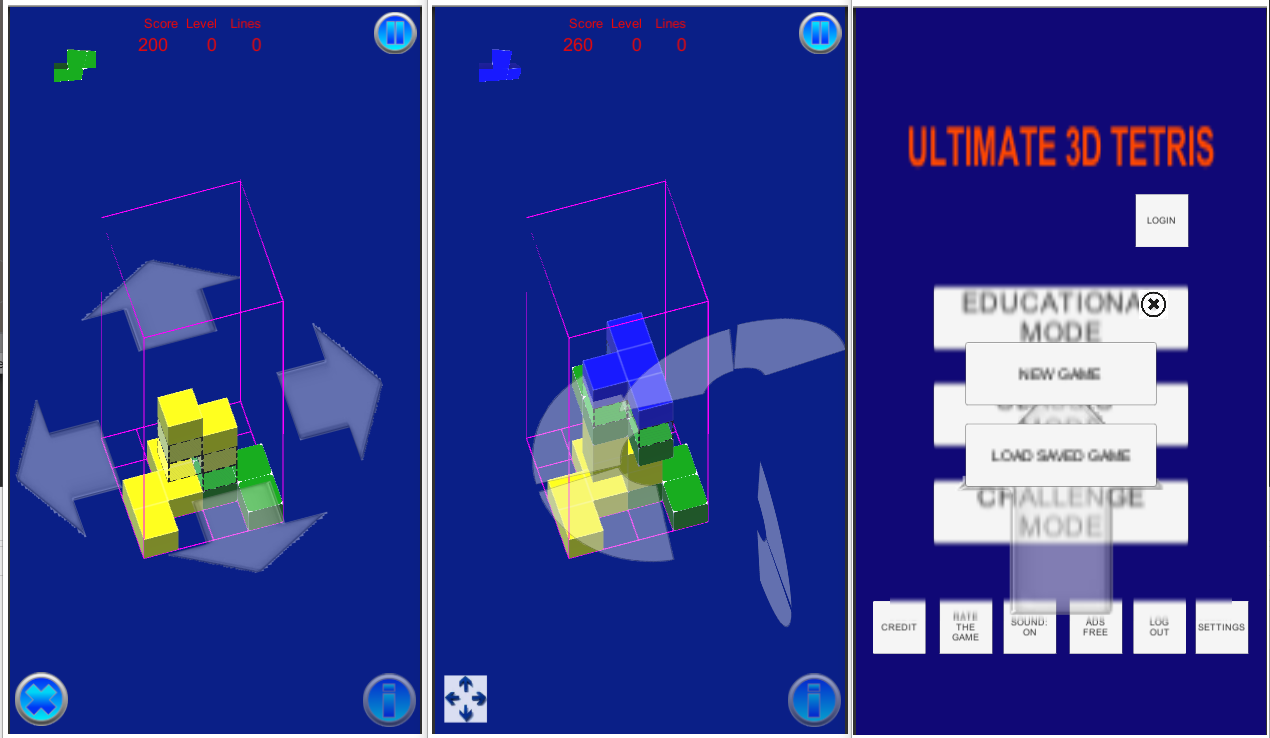
\includegraphics[width=.9\linewidth]{./pic/readme_20221007_195217.png}
\begin{itemize}
\item 现在是热更新的框架到上个周末就搭好了,这一两天忙点儿,必要的游戏场景视图基本搭配到位: 场景的搭建没有任何复杂的地方,只是相机的使用相对不够熟练,所有的都只是场景搭建基本功
\end{itemize}
m
% Emacs 27.1 (Org mode 8.2.7c)
\end{document}